\documentclass[12pt, a4paper]{article}
\usepackage[a4paper, left=2cm, right=2cm, top=3cm, bottom=3cm]{geometry}

\usepackage[english]{babel}
\usepackage[utf8]{inputenc}
\usepackage{fancyhdr}

\usepackage{enumitem}
\usepackage{amsmath}
\usepackage{mathtools}
\usepackage{listings}

\usepackage{array}

\usepackage{tikz}
\usetikzlibrary{arrows.meta,shapes.multipart}

\pagestyle{fancy}
\fancyhf{}
\lhead{Tutorium 02 \\ Abgabegruppe 01}
\chead{Blatt 07 \\ DatKom}
\rhead{Andrés Montoya, 405409 \\ Til Mohr, 405959}

\begin{document}

\begin{center}\fcolorbox{red}{yellow}{\begin{minipage}{35em}
	Bei uns war ursprünglich noch ein Dritter in unserer Abgabegruppe eingeteilt. Wir haben ihn vor über einer Woche versucht per E-Mail zu erreichen, leider erfolglos.\\
	Nach Ablauf der Anmeldefrist zu den Abgabegruppen haben wir gesehen, dass diese Person leider unsere Abgabegruppe verlassen hat.\\
	Bisher konnten wir noch keinen Dritten für unsere Abgabegruppe finden.\\
	Uns wurde auch seit dem letzten Blatt keine weitere Person zugeteilt.
\end{minipage}}\end{center}



\section*{Aufgabe 7.1}
\begin{enumerate}[label=\alph*)]
	\item	Durchgezogene grüne Verbindungen: Geringste Kosten. \\
			LAX-SFO + SFO-JFK + JFK-LHR = LAX-MIA + MIA-LHR für iii). \\
			AMS-CPT $>$ AMS-FRA + FRA+CPT für ii). \\
			MIA-LHR + LHR-AMS + AMS-FRA $<$ MIA-CPT + CPT-FRA für ii). \\
			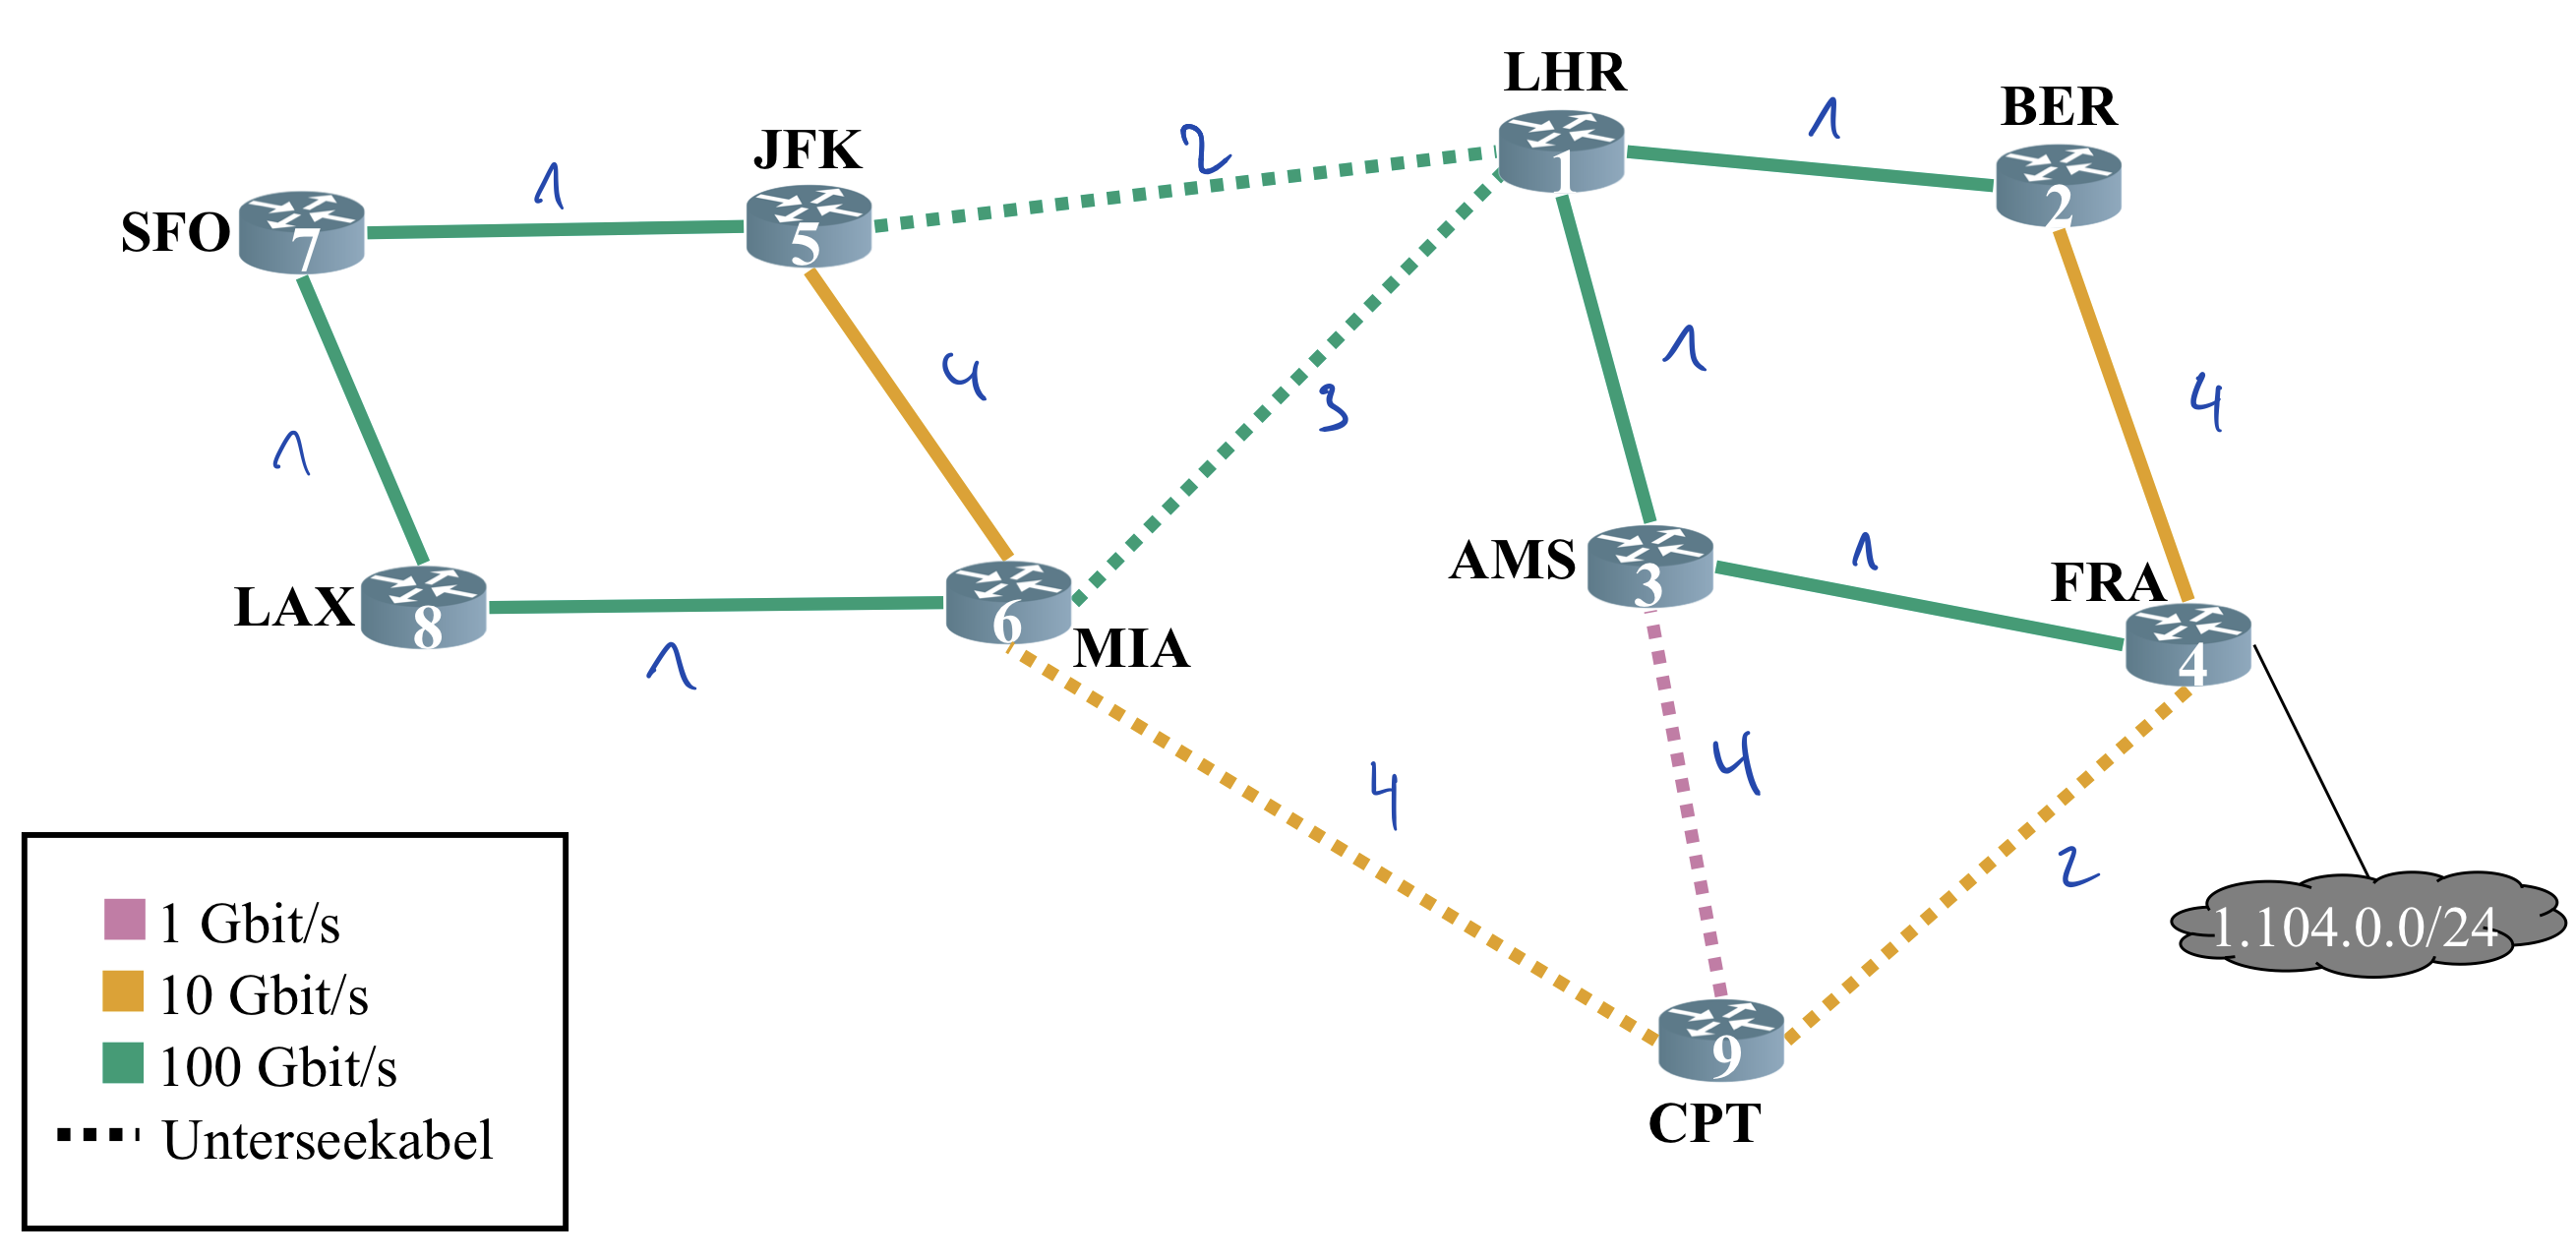
\includegraphics[scale=0.35]{7.1_a).png}
	\item	1.102.0.0/24 via 1.0.1.1 cost 1 \\
			1.103.0.0/24 via 1.0.2.1 cost 1 \\
			1.104.0.0/24 via 1.0.2.1 cost 2 \\
			1.105.0.0/24 via 1.0.5.1 cost 2 \\
			1.106.0.0/24 via 1.0.6.1 cost 3 \\
			1.107.0.0/24 via 1.0.5.1 cost 3 \\
			1.108.0.0/24 via 1.0.5.1 cost 4 \\
			1.108.0.0/24 via 1.0.6.1 cost 4 \\
			1.109.0.0/24 via 1.0.2.1 cost 4 \\
	\item	An MIA muss man die Kosten für 1.0.7.2/24 senken, z.B. auf 1. Zusätzlich müssten wir für Lax die Kosten von 1.0.9.2/24 auf z.B. 2 erhöhen. Damit zwingen wir den Traffic über JFK. \\
			Der Nachteil hierbei ist, dass hierbei die load-balancing-Eigenschaft verloren geht.
\end{enumerate}


\newpage


\section*{Aufgabe 7.2}
\begin{enumerate}[label=\alph*)]
	\item	\newcolumntype{C}[1]{>{\centering\arraybackslash}p{#1}}
			\renewcommand{\arraystretch}{2}
			\begin{center}\begin{tabular}{c||C{1cm}|C{1cm}|C{1cm}|C{1cm}|C{1cm}|C{1cm}|C{1cm}}
					& A & B & C & D & E & F & G \\ 
				\hline\hline
				A 	& - & B,5 & $\infty$ & $\infty$ & $\infty$ & F,7 & G,2 \\ \hline
				B 	& A,5 & - & C,13 & $\infty$ & $\infty$ & $\infty$ & $\infty$ \\ \hline
				C 	& $\infty$ & B,13 & - & D,7 & E,1 & $\infty$ & $\infty$ \\ \hline
				D 	& $\infty$ & $\infty$ & C,7 & - & $\infty$ & $\infty$ & $\infty$ \\ \hline
				E 	& $\infty$ & $\infty$ & C,1 & $\infty$ & - & F,5 & $\infty$ \\ \hline
				F 	& A,7 & $\infty$ & $\infty$ & $\infty$ & E,5 & - & G,12 \\ \hline
				G 	& A,2 & $\infty$ & $\infty$ & $\infty$ & $\infty$ & F,12 & -
			\end{tabular}\end{center}
			\renewcommand{\arraystretch}{2}
	\item	\newcolumntype{C}[1]{>{\centering\arraybackslash}p{#1}}
			\renewcommand{\arraystretch}{2}
			\begin{center}\begin{tabular}{c||C{1cm}|C{1cm}|C{1cm}|C{1cm}|C{1cm}|C{1cm}|C{1cm}}
					& A & B & C & D & E & F & G \\ 
				\hline\hline
				A 	& - & B,5 & B,18 & $\infty$ & F,12 & F,7 & G,2 \\ \hline
				B 	& A,5 & - & C,13 & C,20 & C,14 & A,12 & A,7 \\ \hline
				C 	& B,18 & B,13 & - & D,7 & E,1 & E,6 & $\infty$ \\ \hline
				D 	& $\infty$ & C,20 & C,7 & - & C,8 & $\infty$ & $\infty$ \\ \hline
				E 	& F,12 & C,14 & C,1 & C,8 & - & F,5 & F,17 \\ \hline
				F 	& A,7 & A,12 & E,6 & $\infty$ & E,5 & - & A,9 \\ \hline
				G 	& A,2 & A,7 & $\infty$ & $\infty$ & F,17 & A,9 & -
			\end{tabular}\end{center}
			\renewcommand{\arraystretch}{2}
	\item	\newcolumntype{C}[1]{>{\centering\arraybackslash}p{#1}}
			\renewcommand{\arraystretch}{2}
			\begin{center}\begin{tabular}{c||C{1cm}|C{1cm}|C{1cm}|C{1cm}|C{1cm}|C{1cm}|C{1cm}}
					& A & B & C & D & E & F & G \\ 
				\hline\hline
				A 	& - & B,5 & F,13 & F,20 & F,12 & F,7 & G,2 \\ \hline
				B 	& A,5 & - & C,13 & C,20 & C,14 & A,12 & A,7 \\ \hline
				C 	& B,18 & B,13 & - & D,7 & E,1 & E,6 & E,15 \\ \hline
				D 	& C,20 & C,20 & C,7 & - & C,8 & C,13 & C,22 \\ \hline
				E 	& F,12 & C,14 & C,1 & C,8 & - & F,5 & F,14 \\ \hline
				F 	& A,7 & A,12 & E,6 & E,13 & E,5 & - & A,9 \\ \hline
				G 	& A,2 & A,7 & A,15 & A,22 & A,14 & A,9 & -
			\end{tabular}\end{center}
			\renewcommand{\arraystretch}{2}
\end{enumerate}


\newpage


\section*{Aufgabe 7.3}
\begin{enumerate}[label=\alph*)]
	\item	Vorteil: Entlastung der Router \\
			Nachteil: "Overhead": Dasselbe Paket muss mehrmals gesendet werden + Overhead durch zusätzliche Header für die Fragmente
	\item	Vorteil: Es müssen weniger Daten gesendet werden \\
			Nachteil: Übertragungsfehler müssen in den höheren Schichten abgefangen werden (kann aber auch Vorteil sein, wenn man Paketfehler akzeptiert)
	\item	IPv6 (genauso IPv4) ist immer Standortbezogen durch Netze und Subnetze. Erstellt man also mit seiner MAC-Adresse eine IPv6-Adresse, so ist diese nur im gegebenen Subnetz gebrauchbar. Ändert man seinen Netzzugangspunkt so, dass man sich in einem anderen Subnetz befindet, wird diese IPv6-Adresse ungebrauchbar.
\end{enumerate}


\newpage


\section*{Aufgabe 7.4}
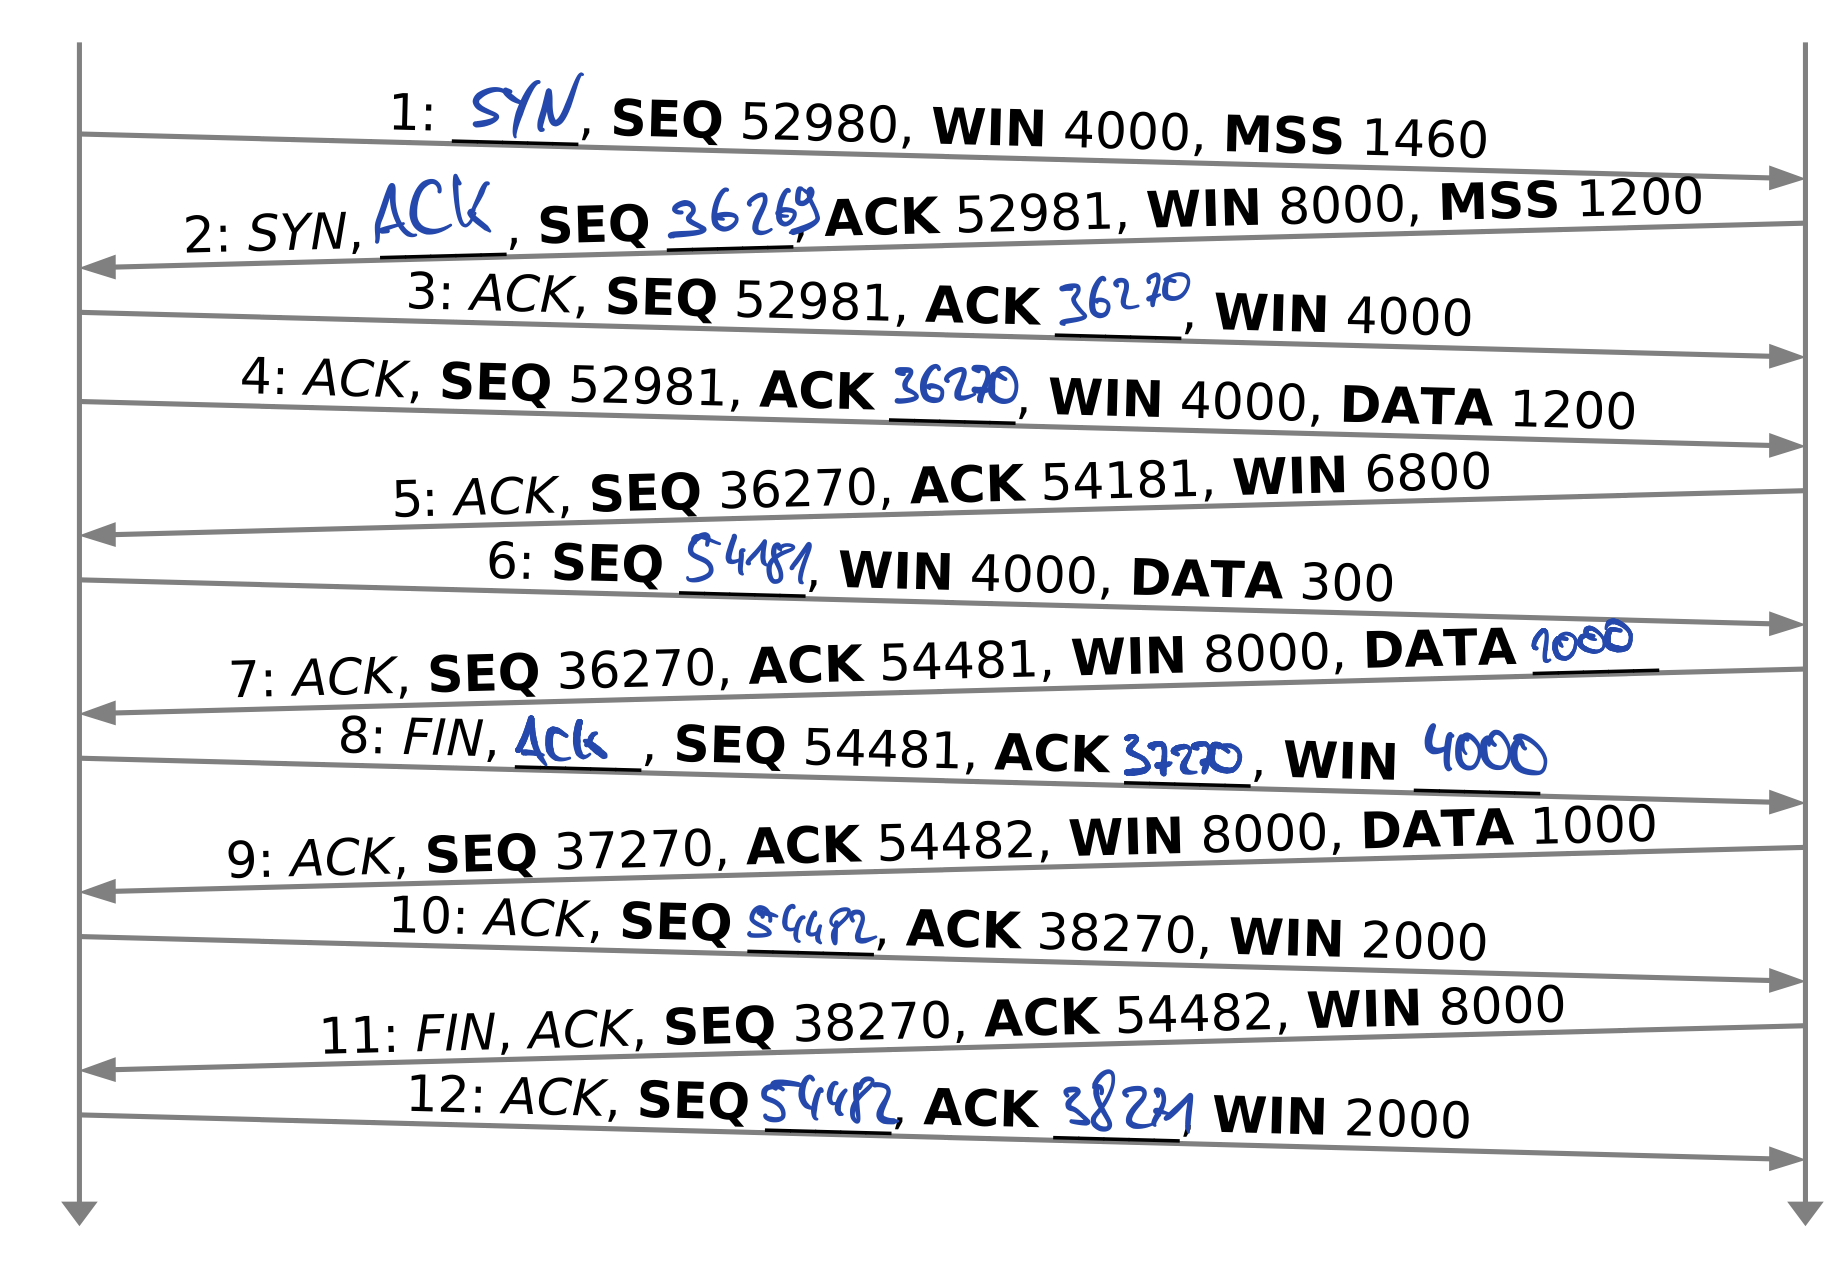
\includegraphics[scale=0.5]{7.4.png}


\end{document}